\begin{figure}[H]
    \centering
    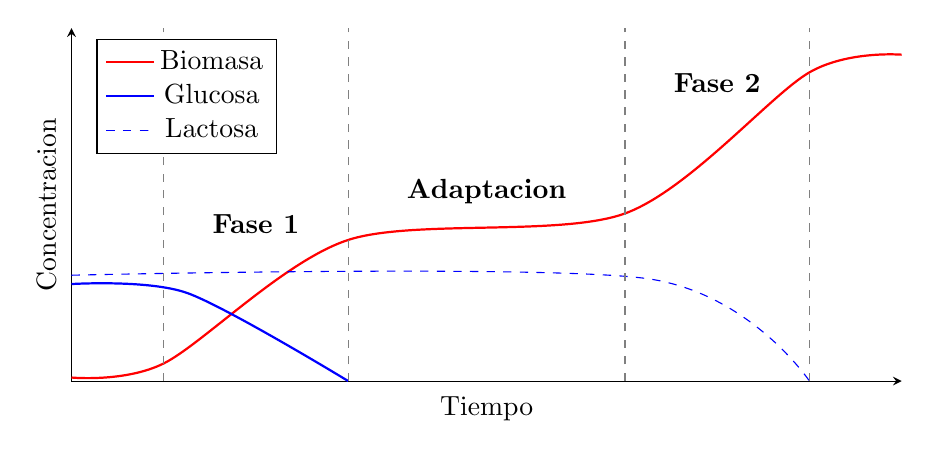
\begin{tikzpicture}
        \begin{axis}[
            width=\linewidth,
            height=0.5\linewidth,
            axis lines = left,
            xlabel = Tiempo,
            xmin=0, xmax=9,
            xtick=\empty,
            ylabel = Concentracion,
            ymin=0, ymax=10,
            ytick=\empty,
            grid=major,
            grid style={dashed, gray!20},
            legend pos=north west,
        ]
        \addplot[thick, red, smooth, tension=0.5] coordinates {
            (0, 0.1)
            (1, 0.5)
            (3, 4)
            (6, 4.75)
            (8, 8.75)
            (9, 9.25)
        };
        \addplot[thick, blue, smooth, tension=0.5] coordinates {
            (0, 2.75)
            (1.25, 2.5)
            (3, 0)
        };
        \addplot[dashed, blue, smooth, tension=0.5] coordinates {
            (0, 3)
            (6.25, 2.9)
            (8, 0)
        };
        \draw[dashed, gray] (1,0) -- (1,10);
        \draw[dashed, gray] (3,0) -- (3,10);
        \draw[dashed, gray] (6,0) -- (6,10);
        \draw[dashed, gray] (8,0) -- (8,10);
        \node[anchor=north] at (2,5) {\textbf{Fase 1}};
        \node[anchor=north] at (4.5,6) {\textbf{Adaptacion}};
        \node[anchor=north] at (7,9) {\textbf{Fase 2}};
        \addlegendentry{\textcolor{black}{Biomasa}}
        \addlegendentry{\textcolor{black}{Glucosa}}
        \addlegendentry{\textcolor{black}{Lactosa}}
        \end{axis}
    \end{tikzpicture}
    
    \rule{\linewidth}{0.2pt}
    \caption[Ejemplo de curva diáuxica]{Ejemplo de curva diáuxica. Se observa una correspondencia entre el consumo de glucosa y la primer fase log, así como del consumo de lactosa y la segunda fase log, así como una fase estacionaria intermedia, esto en el proceso para adaptar la maquinaria enzimática del microorganismo para poder degradar lactosa.}
    \label{fig:curva_diauxica}
\end{figure}